\section{\molmothink}
\label{sec:reasoning}


\begin{figure}[t]
    \centering
    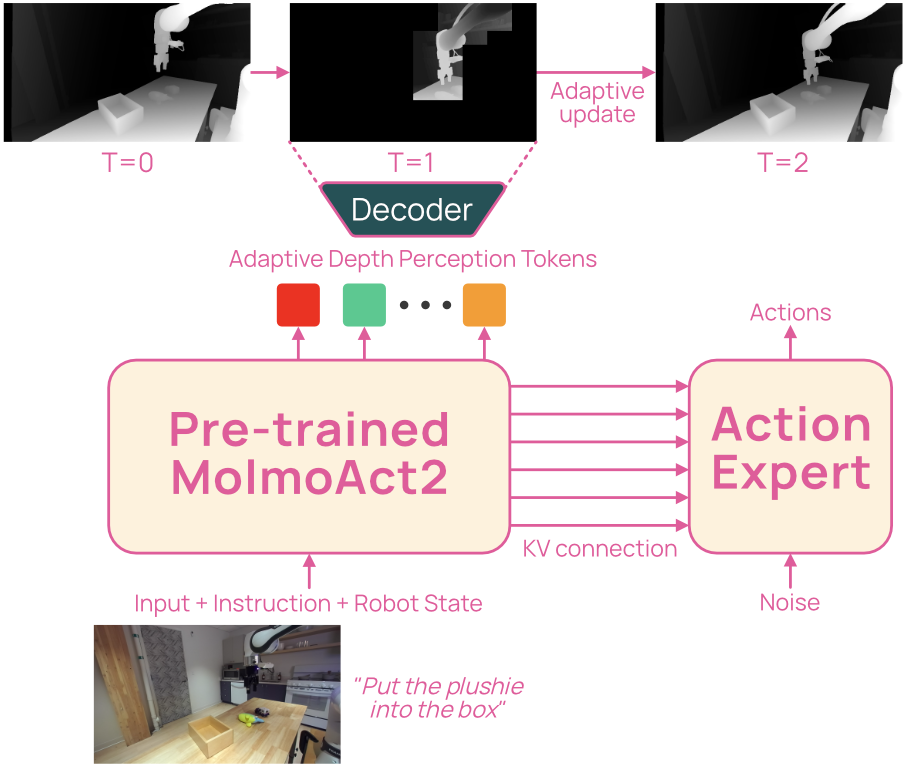
\includegraphics[width=0.6\linewidth]{figures/MAF44.png}
    \caption{\textbf{Overview of \molmothink.} 
\molmothink augments the \molmoactt action-generation pipeline with adaptive 
depth-token reasoning, reusing cached depth codes for static regions and regenerating 
depth codes for changed regions before conditioning the action expert.}
    \label{fig:think-adaptive-depth}
\end{figure}


Robotic manipulation depends on spatial information that is only indirectly
supervised by action imitation: object distance, free space, occlusion, and
surface layout all affect the action, but standard behavior-cloning objectives
do not ask the model to make this structure explicit before acting. \molmoact
\citep{lee2025molmoactactionreasoningmodels} addressed this problem by adding
depth-token prediction as an intermediate reasoning step. \molmothink extends
the same idea to \molmoactt: before producing an action, the model predicts a
compact discrete depth representation that conditions the action expert through
per-layer KV conditioning.

The depth representation is intentionally lightweight. Each observation depth
map is quantized into a \(10 \times 10\) grid, giving 100 spatial code
positions, and each position takes one of 128 learned depth-code values. These
codes are represented as ordinary autoregressive tokens, which makes depth reasoning compatible with the same next-token interface used throughout \molmoactt while exposing an interpretable intermediate prediction.

The main distinction from \molmoact is that \molmothink makes depth prediction
adaptive across time. Robot trajectories contain substantial temporal
redundancy: many cells in a scene-level depth grid remain unchanged from one
control step to the next. Instead of re-predicting every depth code at every
step, \molmothink reuses cached codes for static regions and autoregressively
predicts only the cells whose RGB evidence changes. The result is a
depth-aware policy whose geometric reasoning cost scales with scene change
rather than with the full 100-token grid.

\subsection{Adaptive depth perception data}
\label{sec:think-data}

For every robotics dataset used by \molmothink in the mixtures described in
\autoref{sec:data}, we attach depth annotations to the policy observation
stream. We use the same camera stream that is presented to the policy for depth
reasoning: single-view datasets use their canonical observation camera,
and multi-view datasets use the first policy view with available depth annotations. For heterogeneous LeRobot datasets, when a camera is not specified
explicitly, the video feature is selected from the dataset metadata.

For each RGB frame, we estimate a dense monocular depth map with Depth Anything
V2~\citep{depth_anything_v2}. We then quantize that depth map with the trained
depth VQ-VAE used by \molmoact~\citep{lee2025molmoactactionreasoningmodels},
following the tokenization scheme of \citet{ning2023tokensunifyingoutputspace}.
The VQ-VAE operates on a \(320 \times 320\) depth image with a downsampling
factor of 32, producing a \(10 \times 10\) grid of codebook indices in
\(\{0,\ldots,127\}\).

The same preprocessing pass also constructs the adaptive-depth side channels
used during training and inference. Let \(d_t \in \{0,\ldots,127\}^{100}\) be
the full VQ depth codes for frame \(t\), flattened in raster order. We maintain
a buffer \(b_t\) and update mask \(m_t \in \{0,1\}^{100}\). For the first frame
of an episode, all positions are updated and \(b_1=d_1\). For later frames, the
RGB image is resized to \(320 \times 320\), divided into the same \(10 \times
10\) grid of \(32 \times 32\) patches, and each patch is compared to the
corresponding patch in the previous frame by cosine similarity. A cell is
marked updated when the similarity is below 0.996:
\begin{equation}
    m_{t,i}
    =
    \mathbf{1}
    \left[
        \cos(x_{t,i}, x_{t-1,i}) < 0.996
    \right],
    \qquad
    b_{t,i}
    =
    \begin{cases}
    d_{t,i}, & m_{t,i}=1, \\
    b_{t-1,i}, & m_{t,i}=0.
    \end{cases}
\end{equation}
Thus each frame stores the full depth codes \(d_t\), the carried-forward depth
buffer \(b_t\), and the binary update mask \(m_t\). The model is supervised on
the buffer codes, matching the representation it will maintain during adaptive
inference.

\subsection{Training}
\label{sec:think-training}

\paragraph{Post-training.}
\molmothink starts from the same 200K-step \molmoacttpre checkpoint as the
standard \molmoactt post-training stage. We keep the post-training recipe in
\autoref{sec:posttraining}: the same data construction, action expert, per-layer
KV conditioning, sequence lengths, optimizer settings, 100K training
updates, global batch size of 128, and 64 H100 GPUs. On top of \molmoactt, we added depth-related special tokens for training \molmothink, where the full depth-token interface is in \autoref{supp:model-depth}.

Within robot data, post-training uniformly samples three tasks: action
prediction, depth prediction, and depth-and-action prediction. The action task
trains the usual discrete and continuous action objectives. The depth task
trains autoregressive prediction of the 100 depth-buffer tokens. In the
depth-and-action task, the model first predicts depth tokens, then predicts
discrete action tokens autoregressively while the action expert conditions on
the input context and predicted depth state to generate continuous actions. The
prompt templates and assistant-side triggers for these output styles are given
in \autoref{supp:training}. As in \autoref{sec:posttraining}, the target
action-token span is masked from the expert conditioning path, so the expert
can use the task, observations, state, and depth tokens, but not the discrete
action target it is trained to predict.



\paragraph{Fine-tuning.}
The \molmothinklibero checkpoint is fine-tuned from the depth-aware
post-trained checkpoint using the same full-\libero recipe and compute budget as
\autoref{sec:finetuning}: robot-only training on the combined Spatial, Object,
Goal, and Long suites, with front-view then wrist-view camera order,
2100-token sequences, global batch size 64, 32 H100 GPUs, and 50K updates. We select the
best checkpoint at 30K updates for evaluation.

Fine-tuning differs from depth post-training in three targeted ways. First, we
sample only action and depth-and-action examples, again uniformly, and remove
the pure depth-prediction style. Second, because inference conditions on depth
tokens predicted by the model rather than oracle depth tokens, we inject noise
into the teacher-forced depth prefix during training: 10\% of depth-code input
tokens are replaced by uniformly sampled depth codes, while the prediction
targets remain unchanged. Third, we add a learned per-layer gate on the depth
portion of the action expert's per-layer KV conditioning. For action-expert layer
\(\ell\), let \(M_t=1\) denote positions belonging to the depth-output trigger,
depth delimiters, or depth-code tokens, and let \(A_t\) denote valid context
positions. The gate is computed from the non-depth context of the corresponding
VLM layer,
\begin{equation}
    c_\ell
    =
    \frac{
        \sum_t A_t(1-M_t)V^{\mathrm{vlm}}_{\ell,t}
    }{
        \sum_t A_t(1-M_t)
    },
    \qquad
    g_\ell
    =
    \sigma(w_\ell^\top c_\ell + b_\ell),
\end{equation}
and then applied only to depth-token keys and values:
\begin{equation}
    \bar{K}^{\mathrm{vlm}}_{\ell,t}
    =
    \left(1-M_t+M_t g_\ell\right)K^{\mathrm{vlm}}_{\ell,t},
    \qquad
    \bar{V}^{\mathrm{vlm}}_{\ell,t}
    =
    \left(1-M_t+M_t g_\ell\right)V^{\mathrm{vlm}}_{\ell,t}.
\end{equation}
The gated \((\bar{K}^{\mathrm{vlm}}_{\ell},\bar{V}^{\mathrm{vlm}}_{\ell})\)
are then projected into the action expert as in \autoref{sec:posttraining}.
The gate is initialized with bias \(-4\), so fine-tuning begins close to the
standard action-conditioning path and learns how strongly each expert layer
should use the depth prefix. Additional model-level details for the depth
extension are summarized in \autoref{supp:model-depth}.

\subsection{Adaptive depth inference}
\label{sec:adaptive-depth-inference}

\paragraph{Inference pipeline.}
At inference, \molmothink uses the depth-and-action output style. Given the task,
current observation, and proprioceptive state, the prompt requests
\texttt{<depth\_output><action\_output>}. The model first performs a prefill
over the prompt and images. If no depth cache is available, as at the beginning
of a rollout or after a reset, it autoregressively predicts the full depth
sequence: \texttt{<depth\_start>}, 100 depth-code tokens, and
\texttt{<depth\_end>}.

When a depth cache is available, the model compares the current first
observation image to the cached previous image using the same \(10 \times 10\)
RGB-patch cosine threshold described in \autoref{sec:think-data}. Updated cells
are generated by argmax decoding from the depth-token logits. Unchanged cells
are replayed from the previous predicted depth buffer and consumed by the model
as known depth-token inputs. Consecutive unchanged spans are replayed together,
whereas changed spans are decoded token by token. After all 100 cells are
filled, the model emits \texttt{<depth\_end>} and stores the current image and
the newly filled 100-code depth buffer as the cache for the next control step.

The action is then generated from the depth-conditioned state. For continuous
control, the action expert receives the VLM keys and values corresponding to
the prompt plus the filled depth prefix and integrates the flow-matching
velocity field to produce the action chunk. Adaptive depth changes only how the intermediate depth prefix is produced. The
action interface remains the same as the depth-and-action training objective.



\paragraph{Inference optimization.}
Adaptive depth inference introduces a different systems challenge from the continuous action expert: each frame can contain a different mixture of regenerated depth cell and replayed cached cells, so the overall decode schedule is data-dependent. Capturing the full adaptive loop would require a separate graph for each update pattern. We therefore keep the adaptive scheduler eager, including span-level replay for unchanged cells, while using a preallocated static KV cache to make the decode state stable across steps. For regenerated depth tokens, we capture the fixed-shape transformer work from post-attention through the next layer's pre-attention as CUDA Graph stages, and leave attention itself eager because its effective KV length changes throughout decoding. This preserves adaptive depth reuse while reducing the launch bubbles in the repeated one-token decode path.



\begin{table*}[t]
    \caption{\textbf{Embodied reasoning results.} We evaluate on benchmarks across spatial reasoning, pointing, and embodied QA tasks. The best-performing open-weight model on each benchmark is in \textbf{bold}, and the second best is \underline{underlined}.}
    \renewcommand{\arraystretch}{1.15}
    \setlength{\tabcolsep}{3pt}
    \centering
    \resizebox{\textwidth}{!}{%
    \begin{tabular}{@{}lcccccccccccccc@{}}
        % \toprule
        \textbf{\large Models/Benchmarks} &
        \rotatebox{90}{\shortstack{\textbf{\large Point-Bench} \\ \citep{cheng2025pointarena}}} &
        \rotatebox{90}{\shortstack{\textbf{\large RefSpatial} \\ \citep{zhou2025roborefer}}} &
        \rotatebox{90}{\shortstack{\textbf{\large RoboSpatial-Poi} \\ \citep{song2025robospatial}}} &
        \rotatebox{90}{\shortstack{\textbf{\large Where2Place} \\ \citep{yuan2024robopoint}}} &
        \rotatebox{90}{\shortstack{\textbf{\large BLINK} \\ \citep{fu2024blink}}} &
        \rotatebox{90}{\shortstack{\textbf{\large CV-Bench} \\ \citep{tong2024cambrian}}} &
        \rotatebox{90}{\shortstack{\textbf{\large ERQA} \\ \citep{team2025gemini}}} &
        \rotatebox{90}{\shortstack{\textbf{\large EmbSpatial} \\ \citep{du2024embspatial}}} &
        \rotatebox{90}{\shortstack{\textbf{\large MindCube} \\ \citep{luopyspatial}}} &
        \rotatebox{90}{\shortstack{\textbf{\large RoboSpatial-VQ} \\ \citep{song2025robospatial}}} &
        \rotatebox{90}{\shortstack{\textbf{\large SAT} \\ \citep{ray2025satdynamicspatialaptitude}}} &
        \rotatebox{90}{\shortstack{\textbf{\large OpenEQA} \\ \citep{majumdar2024openeqa}}} &
        \rotatebox{90}{\shortstack{\textbf{\large VSI-Bench} \\ \citep{yang2025thinking}}} &
        \rotatebox{90}{\textbf{\large Overall Avg.}} \\
        \midrule
        \multicolumn{15}{@{}l}{\textbf{\textit{\large API call only}}} \\
        {\large GR-ER 1.5 Thinking~\citep{team2025gemini}} & {\large 71.6} & {\large 48.5} & {\large 31.1} & {\large 59.0} & {\large 57.8} & {\large 84.3} & {\large 54.8} & {\large 78.4} & {\large 54.7} & {\large 79.3} & {\large 76.7} & {\large 55.0} & {\large 45.8} & {\large 61.3} \\
        {\large GR-ER 1.5~\citep{team2025gemini}}          & {\large 73.3} & {\large 41.8} & {\large 25.3} & {\large 48.0} & {\large 65.2} & {\large 83.6} & {\large 47.0} & {\large 73.4} & {\large 47.7} & {\large 57.0} & {\large 62.0} & {\large 50.5} & {\large 39.9} & {\large 55.0} \\
        {\large Gemini 2.5 Pro~\citep{comanici2025gemini}} & {\large 62.7} & {\large 33.6} & {\large 8.3} & {\large 37.0} & {\large 69.2} & {\large 85.9} & {\large 56.0} & {\large 78.0} & {\large 59.2} & {\large 71.3} & {\large 74.7} & {\large 55.0} & {\large 51.1} & {\large 57.1} \\
        {\large GPT-5~\citep{singh2025openai}}             & {\large 43.6} & {\large 23.5} & {\large 19.0} & {\large 37.0} & {\large 71.3} & {\large 86.1} & {\large 59.0} & {\large 81.5} & {\large 58.0} & {\large 69.3} & {\large 86.7} & {\large 64.4} & {\large 52.9} & {\large 57.9} \\
        {\large GPT-5-mini ~\citep{singh2025openai}}       & {\large 39.5} & {\large 23.0} & {\large 12.5} & {\large 33.5} & {\large 56.4} & {\large 85.9} & {\large 57.3} & {\large 78.8} & {\large 55.6} & {\large 70.7} & {\large 81.3} & {\large 59.2} & {\large 46.2} & {\large 53.8} \\
        \midrule
        \multicolumn{15}{@{}l}{\textbf{\textit{\large Open weights only}}} \\
        {\large Qwen3-VL-4B~\citep{qwen3}}                 & {\large 63.8} & {\large \underline{49.5}} & \textbf{\large 62.3} & \textbf{\large 63.0} & {\large 65.2} & \underline{\large 85.8} & {\large 39.5} & {\large 78.1} & {\large 27.4} & {\large 62.7} & {\large 60.7} & \underline{\large 47.6} & {\large 61.4} & {\large 59.0} \\
        {\large Qwen3-VL-8B~\citep{qwen3}}                 & {\large 64.2} & {\large 47.5} & \underline{\large 56.6} & \textbf{\large 63.0} & \underline{\large 66.6} & {\large 85.6} & {\large 41.5} & \underline{\large 78.2} & {\large 33.4} & \textbf{\large 73.7} & \underline{\large 70.0} & \textbf{\large 49.3} & \underline{\large 63.3} & \underline{\large 61.0} \\
        {\large LLaVA-OV-7B~\citep{li2024llava}}           & {\large 9.4} & {\large 3.0} & {\large 0.0} & {\large 19.0} & {\large 44.2} & {\large 70.3} & {\large 39.8} & {\large 69.7} & \underline{\large 45.6} & {\large 68.9} & {\large 58.0} & {\large 36.2} & {\large 31.2} & {\large 38.1} \\
        {\large InternVL3.5-4B~\citep{wang2025internvl3}}  & {\large 43.0} & {\large 21.5} & {\large 23.0} & {\large 53.0} & {\large 58.7} & {\large 80.5} & {\large 37.0} & {\large 72.0} & {\large 42.6} & {\large 61.0} & {\large 49.3} & {\large 44.6} & {\large 56.5} & {\large 49.4} \\
        {\large InternVL3.5-8B~\citep{wang2025internvl3}}  & {\large 45.5} & {\large 35.0} & {\large 27.0} & \underline{\large 57.0} & {\large 59.1} & {\large 80.9} & {\large 41.0} & {\large 74.7} & {\large 39.7} & {\large 62.7} & {\large 58.7} & {\large 43.5} & {\large 56.4} & {\large 52.4} \\
        \midrule
        \multicolumn{15}{@{}l}{\textbf{\textit{\large Molmo family: Open weights, Open data, Open code}}} \\
        {\large Molmo2 ~\citep{clark2026molmo2openweightsdata}}                                 & \underline{\large 76.9} & \textbf{\large 52.5} & {\large 13.9} & {\large 18.0} & {\large 50.8} & {\large 64.4} & \underline{\large 46.3} & {\large 67.0} & {\large 37.6} & {\large 57.9} & {\large 50.0} & {\large 46.9} & {\large 26.1} & {\large 46.8} \\
        {\color{ai2pink} \large \molmoer}                              & \textbf{\large 77.3} & \textbf{\large 52.5} & {\large 32.0} & {\large 54.0} & \textbf{\large 72.5} & \textbf{\large 87.8} & \textbf{\large 46.8} & \textbf{\large 78.8} & \textbf{\large 57.0} & \underline{\large 73.4} & \textbf{\large 78.0} & {\large 44.7} & \textbf{\large 74.5} & \textbf{\large 63.8} \\
        % \bottomrule
    \end{tabular}%
    }
    \label{tab:er_results}
\end{table*}
